\documentclass[14pt, a4paper]{extarticle}
% Русская локализация
\usepackage[english,russian]{babel}


\usepackage{appendix}
\usepackage{alphabeta}

% Использование математических шрифтов
\usepackage{unicode-math}

% Шрифты
\usepackage{fontspec}
\usepackage{courier}
\defaultfontfeatures{Ligatures={TeX},Renderer=Basic}
\setmainfont[Ligatures={TeX}]{Times New Roman}
\setmonofont{Courier New}
\setmathfont{XITS Math}

% Расширенные ссылки
\usepackage{nameref}

% Оформление URL
\usepackage{xurl}
\usepackage{hyperref}
\hypersetup{
  colorlinks,
  citecolor=black,
  filecolor=black,
  linkcolor=black,
  urlcolor=black,
  breaklinks=true,
}
\urlstyle{same}

% Поддержка изображений
\usepackage{graphicx}
\graphicspath{{./images/}}
\DeclareGraphicsExtensions{.jpg,.png}
\usepackage{svg}

% Таблицы
\usepackage{tabularx}
\usepackage{tabulary}
\usepackage{ltablex}
\usepackage{multirow}
\usepackage{hhline}
% Выравнивание по левому краю, с многострочностью
\newcolumntype{s}{>{\raggedright\arraybackslash}X}

% Поддержка листингов
\usepackage{listings}
\lstdefinestyle{gost}{
  basicstyle=\ttfamily\footnotesize,
  breakatwhitespace=false,
  breaklines=true,
  keepspaces=true,
  showspaces=false,
  showstringspaces=false,
  frame=single
}
\lstset{style=gost}%

% Отступ первой строки первого абзаца
\usepackage{indentfirst}
\linespread{1.25}

% Размер полей в документе
\usepackage{geometry}
\geometry{left=3cm}
\geometry{right=1cm}
\geometry{top=2cm}
\geometry{bottom=2cm}

% Абзацный отступ
\setlength{\parindent}{1.25cm}

% Отступ для элементов в списке
\usepackage{enumitem}
\setlist{left=\parindent, labelsep=1cm, itemsep=0pt, topsep=0pt}

% Загрузка pdf-документов (нужно для титульных листов)
\usepackage[final]{pdfpages}
% Возможность поворота pdf файло
\usepackage{pdflscape}
\usepackage{everypage}

\newcommand{\Lpagenumber}{\ifdim\textwidth=\linewidth\else\bgroup%
    \dimendef\margin=0 %use \margin instead of \dimen0
    \ifodd\value{page}\margin=\oddsidemargin
    \else\margin=\evensidemargin%
    \fi

\raisebox{\dimexpr-\topmargin-\headheight-\headsep-0.5\linewidth}[0pt][0pt]{%
      \rlap{\hspace{\dimexpr-\margin+\textheight+\footskip}%
        \llap{\rotatebox{90}{\thepage}}}}%
    \egroup\fi}
\AddEverypageHook{\Lpagenumber}%

\usepackage{float}
% Форматирование подписей
\usepackage{caption}

\usepackage{newfloat}
% \DeclareCaptionType{listing}

\DeclareCaptionLabelSeparator{emdash}{\;\textemdash\;}
\captionsetup[figure]{name={Рисунок}, labelsep=emdash, justification=centering,
position=above, singlelinecheck=off, font={small, bf}, labelfont=bf, skip=6pt}
\captionsetup[table]{name={Таблица}, labelsep=emdash,
justification=raggedright, position=top, singlelinecheck=off, font={small, it},
labelfont=it, skip=6pt, margin=0cm}
% \captionsetup[lstlisting]{labelsep=emdash, justification=raggedright,
% position=top, singlelinecheck=off, font={small, it}, labelfont=it, skip=6pt,
% margin=0cm}

% Нумеровать внутри заголовков первого уровня
\counterwithin{figure}{section}
\counterwithin{table}{section}
% \counterwithin{lstlisting}{section}
\AtBeginDocument{\counterwithin{lstlisting}{section}}

% Отключение переносов текста
\usepackage{ragged2e}
\justifying
\tolerance=500
\hyphenpenalty=10000
\emergencystretch=3em

% Форматирование заголовков
\usepackage{titlesec}
% Оформление заголовка первого уровня
% Полужирное начертание
% Кегль 18 пт
% С новой страницы
\titleformat{\section}[block]
{\newpage\bfseries\fontsize{18pt}{21.6pt}\selectfont}
{\thesection}
{1em}{}
% Оформление ненумерованных заголовков (Введение, Содержание, список
% источников, и.т.д.)
\titleformat{name=\section,numberless}[block]
{\centering\newpage\bfseries\fontsize{18pt}{21.6pt}\selectfont}
{}
{0em}{}{}
% Отступы у заголовков первого уровня
\titlespacing{\section}
{\parindent}% отступ слева (равен 1.25 см, как у отступа первой строки абзаца)
{0em}% интервал перед
{10mm}% интервал после
% Оформление заголовков второго уровня
\titleformat{\subsection}[block]
{\bfseries\fontsize{16pt}{19.2pt}\selectfont}
{\thesubsection}
{1em}{}
% Отступы у заголовков второго уровня
\titlespacing{\subsection}
{\parindent}% пробел слева
{15mm}% отступ перед
{10mm}% отступ после
% Оформление заголовков второго уровня
\titleformat{\subsubsection}[block]
{\bfseries\selectfont}
{\thesubsection}
{1em}{}
% Отступы у заголовков второго уровня
\titlespacing{\subsubsection}
{\parindent}% пробел слева
{15mm}% отступ перед
{10mm}% отступ после


% Оформление заголовков в содержании
\usepackage{titletoc}
\contentsmargin{0pt}
\renewcommand\contentspage{\thecontentspage}
\dottedcontents{section}[2.3em]{}{2.3em}{5pt}
\dottedcontents{subsection}[2.3em]{}{2.3em}{5pt}
% Оформление приложений
\usepackage{appendix}
\renewcommand\appendixpagename{ПРИЛОЖЕНИЯ}

% Подключение biblatex, с использованием стиля gost-numeric
\usepackage[
citestyle=gost-numeric,
style=gost-numeric,
blockpunct=emdash,
backend=biber,
sorting=none
]{biblatex}
% Запрет разрыва url ссылок
\defcounter{biburlnumpenalty}{3000}
\defcounter{biburlucpenalty}{6000}
\defcounter{biburllcpenalty}{9000}
% Добавление полей для ссылок и даты обращения к ним
\DeclareFieldFormat{url}{Режим доступа: #1}
\DeclareFieldFormat{urldate}{(Дата обращения: #1)}
\renewcommand*{\entrysetpunct}{\par\nopunct\!\!}
% Использовать prac.bib как источник
\addbibresource{diploma.bib}
% Форматирование заголовка библиографии
\defbibheading{bibliography}[\bibname]{%
  \section*{\centering #1}%
  \markboth{#1}{#1}}
  
\usepackage{etoolbox}
\AtBeginEnvironment{tabularx}{\fontsize{12pt}{14pt}\selectfont}


\usepackage{lipsum}
\usepackage{csquotes}

\begin{document}
\def\contentsname{СОДЕРЖАНИЕ}

% Загрузка титула
% \pagenumbering{gobble}
% \begin{titlepage}
%   
\includepdf{title}
%   
\includepdf[pages={1-5}]{title}
% \end{titlepage}
% \pagenumbering{arabic}
% \setcounter{page}{7}

\setcounter{page}{1}
% Содержание
\tableofcontents

\section*{ВВЕДЕНИЕ}
\phantomsection
\addcontentsline{toc}{section}{ВВЕДЕНИЕ}

Исследуемым объектом в рамках проекта является сервис хранения и обработки
данных модуля потребительского кредитования. Этот модуль включает в
себя ответственность за управление ипотечными и кредитными продуктами, так же
за хранение и обработку данных клиентов и генерацию отчетов, как по клиентам
так и работе модуля.

Актуальность темы исследования обусловлена стремительным развитием информационных
технологий и их внедрением во все сферы социально-экономической жизни, включая сектор
финансовых технологий. Кредитные организации в настоящее время находятся в условиях
сильной конкуренции, а это вынуждает активно внедрять новые технологии, в частности
цифровые технологии, которые позволяют оптимизировать затраты и внутренние процессы,
повышать качество обслуживания клиентов и обеспечивать устойчивость бизнес-моделеи.
В этом ключе важное значение приобретает проектирование и фунциольное моделирование
ИТ-инфраструктуры одного из ключевых элементов, который обеспечивает эффективаность
функционирования автоматизированных кредитных систем, а именно модуля потребительского
кредитования.

В отечественной и зарубежной литературе существует много работ, рассматриващих
проблемы проектирования и моделирования ИТ-инфраструктуры в которых так же
рассматриваются архитектурные подходы, выбор технических решений и методы оптимизации
процессов. Однако в условиях быстро меняющейся регулятороной и потребительской среды
задача создания адаптированной, масштабируемой и безопасной ИТ-инфраструктуры с учетом
специфики бизнес-процессов конкретной организации остается актуальной.

Целью данной работы является проектирование и функциональное моделирование
ИТ-инфраструктуры, поддерживающей модуль потребительского кредитования в
кредитной организации, включающего описание архитектуры и обоснование выбранного
программно-аппаратного решения.

Для достижения поставленной цели в работе решаются следующие задачи:

\begin{enumerate}
  \item Анализ вариантов поставки информационно-технологического сервиса;
  \item Анализ вариантов компонентов ИТ-инфраструктуры и обоснование выбранного варианта;
  \item Выбор системного программного обеспечения;
  \item Моделирование топологии развертывания;
  \item Составление спецификации рабочих станций;
  \item Моделирование топологии развертывания инструментального программного обеспечения;
  \item Анализ сетевой инфраструктуры и моделирование сетевой топологии.
\end{enumerate}

Практическая значимость работы заключается в возможности использования представленных
разработок для модернизации или внедрения модулей автоматизированных систем
потребительского кредитования в ИТ-инфраструктуру кредитных организаций, что
способствует повышению надежности, безопасности, отказаустойчивости и производительности.

\section*{ГЛОССАРИЙ}
\phantomsection
\addcontentsline{toc}{section}{ГЛОССАРИЙ}
\begin{raggedright}
  VPC --- Virtual Private Cloud (виртуальная частная сеть). \\
  ЦОД --- Центр обработки данных. \\
  СХД --- Система хранения данных. \\
  СУБД --- Система управления базами данных. \\
  FC --- Fiber Channel (оптоволоконный канал). \\
  ИТ --- Информационные технологии. \\
  ИТ-инфраструктура --- Информационно-технологическая инфраструктура. \\
  UML --- Unified Modeling Language (Унифицированный язык моделирования) \\
\end{raggedright}

\section{ПРОИЗВОДСТВЕННАЯ ПРАКТИКА}

\subsection{Анализ вариатнов поставки информационно-технологического сервиса}

В работе произведен анализ четырех вариантов поставки
информационно-технологического сервиса, который включает в себя выбор между
такими вариантами поставки, как полностью самостоятельный, облачный (SaaS, Paas, IaaS),
мульти-облачный и гибридный. На основе анализа выбран, как самый оптимальный вариант
поставки, полностью самостоятельный вариант.

Полностью облачный сервис \cite{micrasoft-azure-book} по одному из моделей SaaS,
PaaS или IaaS, позволяет снизить затраты на создержание и поддержку ИТ-инфраструктуры,
но не является лучшим решением, так как вводит за собой ряд ограничений, таких как
сильная зависимость от поставщика, ограниченные возможности кастомизации и настройки,
а также, что является критичным, возможные проблемы с безопасностью и сохранностью данных.

Мульти-облачный вариант, подразумевает под собой так же использование облачной
инфраструктуры, но в отличие от полностью облачного варианта, позволяет использовать
разные облачные решения от разных поставщиков, что позволяет избежать
некоторых проблем, связанных с безопасностью и кастомизацией. Однако, данный
вариант так же не является оптимальным, так как требует высококвалифицированных
специалистов для поддержки и настройки, а так же имеет риски конфликтов совместимости,
что существенно сказывается на затратах.

Гибридный подход позволяет совместное исопльзование облачных решений и собственных
ресурсов. Такой вариант позволяет наиболее гибко и без особых затруднений масштабировать
инфраструктуру, но является более дорогим в долгосрочной перспективе, не исключает
пенно данный подход явялется наиболее гибким, чтобы отвечать всем требованиям
регуляторов и требованиям сранения персональных данных, например, Федеральный закона
№152-ФЗ <<О персональных данных>>.

В Таблице\;\ref{tab:infra_options} приведено сравнение всех четырех вариантов поставки
инфраструктуры. Таблица позволяет точечно рассмотреть все возможные варианты, их
преимущества и недостатки.

\begin{tabularx}{\textwidth}{|l|X|X|}
  \caption{Сравнение вариантов поставки ИТ-инфраструктуры\label{tab:infra_options}} \\
  \hline
  Вариант поставки            & Преимущества & Недостатки                           \\\hline
  \endfirsthead
  \caption*{Продолжение таблицы~\ref{tab:infra_options}}                            \\
  \hline
  Вариант поставки            & Преимущества & Недостатки                           \\\hline
  \endhead
  \endfoot
  \endlastfoot

  Полностью самостоятельный   &
  Частный контроль над чувствительныи данными и инфраструктурой;
  отсутствие зависимости от облачных поставщиков;
  гибгость в соответствии требованиям регуляторов (например, 152-ФЗ).
                              &
  Высокие первоначальные затраты на развертывание;
  необходимость содержания ИТ-персонала;
  более длительное внедрение.                                                       \\\hline

  Облачный (SaaS, PaaS, IaaS) &
  Более низкие затраты на поддержку и обслуживание;
  быстрое масштабирование и внедрение;
  меньшая потребность в локальных ресурсах.
                              &
  Сильная зависимость от поставщика;
  ограниченные возможности настройки;
  риски утечки данных и проблемы с безопасностью.                                   \\\hline

  Мульти-облачный             &
  Снижение зависимости от одного поставщика;
  гибкость в выборе сервисов;
  потенциально лучшая безопасность.
                              &
  Необходимость высококвалифицированного персонала;
  риски несовместимости решений;
  повышенные затраты на администрирование;
  риски утечки данных и проблемы с безопасностью.                                   \\

  Гибридный                   &
  Гибкость масштабирования;
  возможность совмещать преимущества облака и локальной инфраструктуры;
  частичный контроль над критичными компонентами.
                              &
  Более высокая стоимость в долгосрочной перспективе;
  повышенные затраты на администрирование;
  не исключены риски утечки данных; сложность интеграции компонентов.               \\\hline
\end{tabularx}

На основе описанных выше данных становится понятно, что для модуля потребительского кредитования
оптимальным вариантом является полностью самостоятельный вариант поставки, так как он позволяет
иметь полный контроль над данными и инфраструктурой, окупается в долгосрочной песпектие, не
требует высококвалифицированного персонала и позволяет избежать проблем с безопасностью.
Диаграмма развертывания в нотации UML представлена на Рисунке\;\ref{fig:infra1}.

\begin{figure}[H]
  \centering
  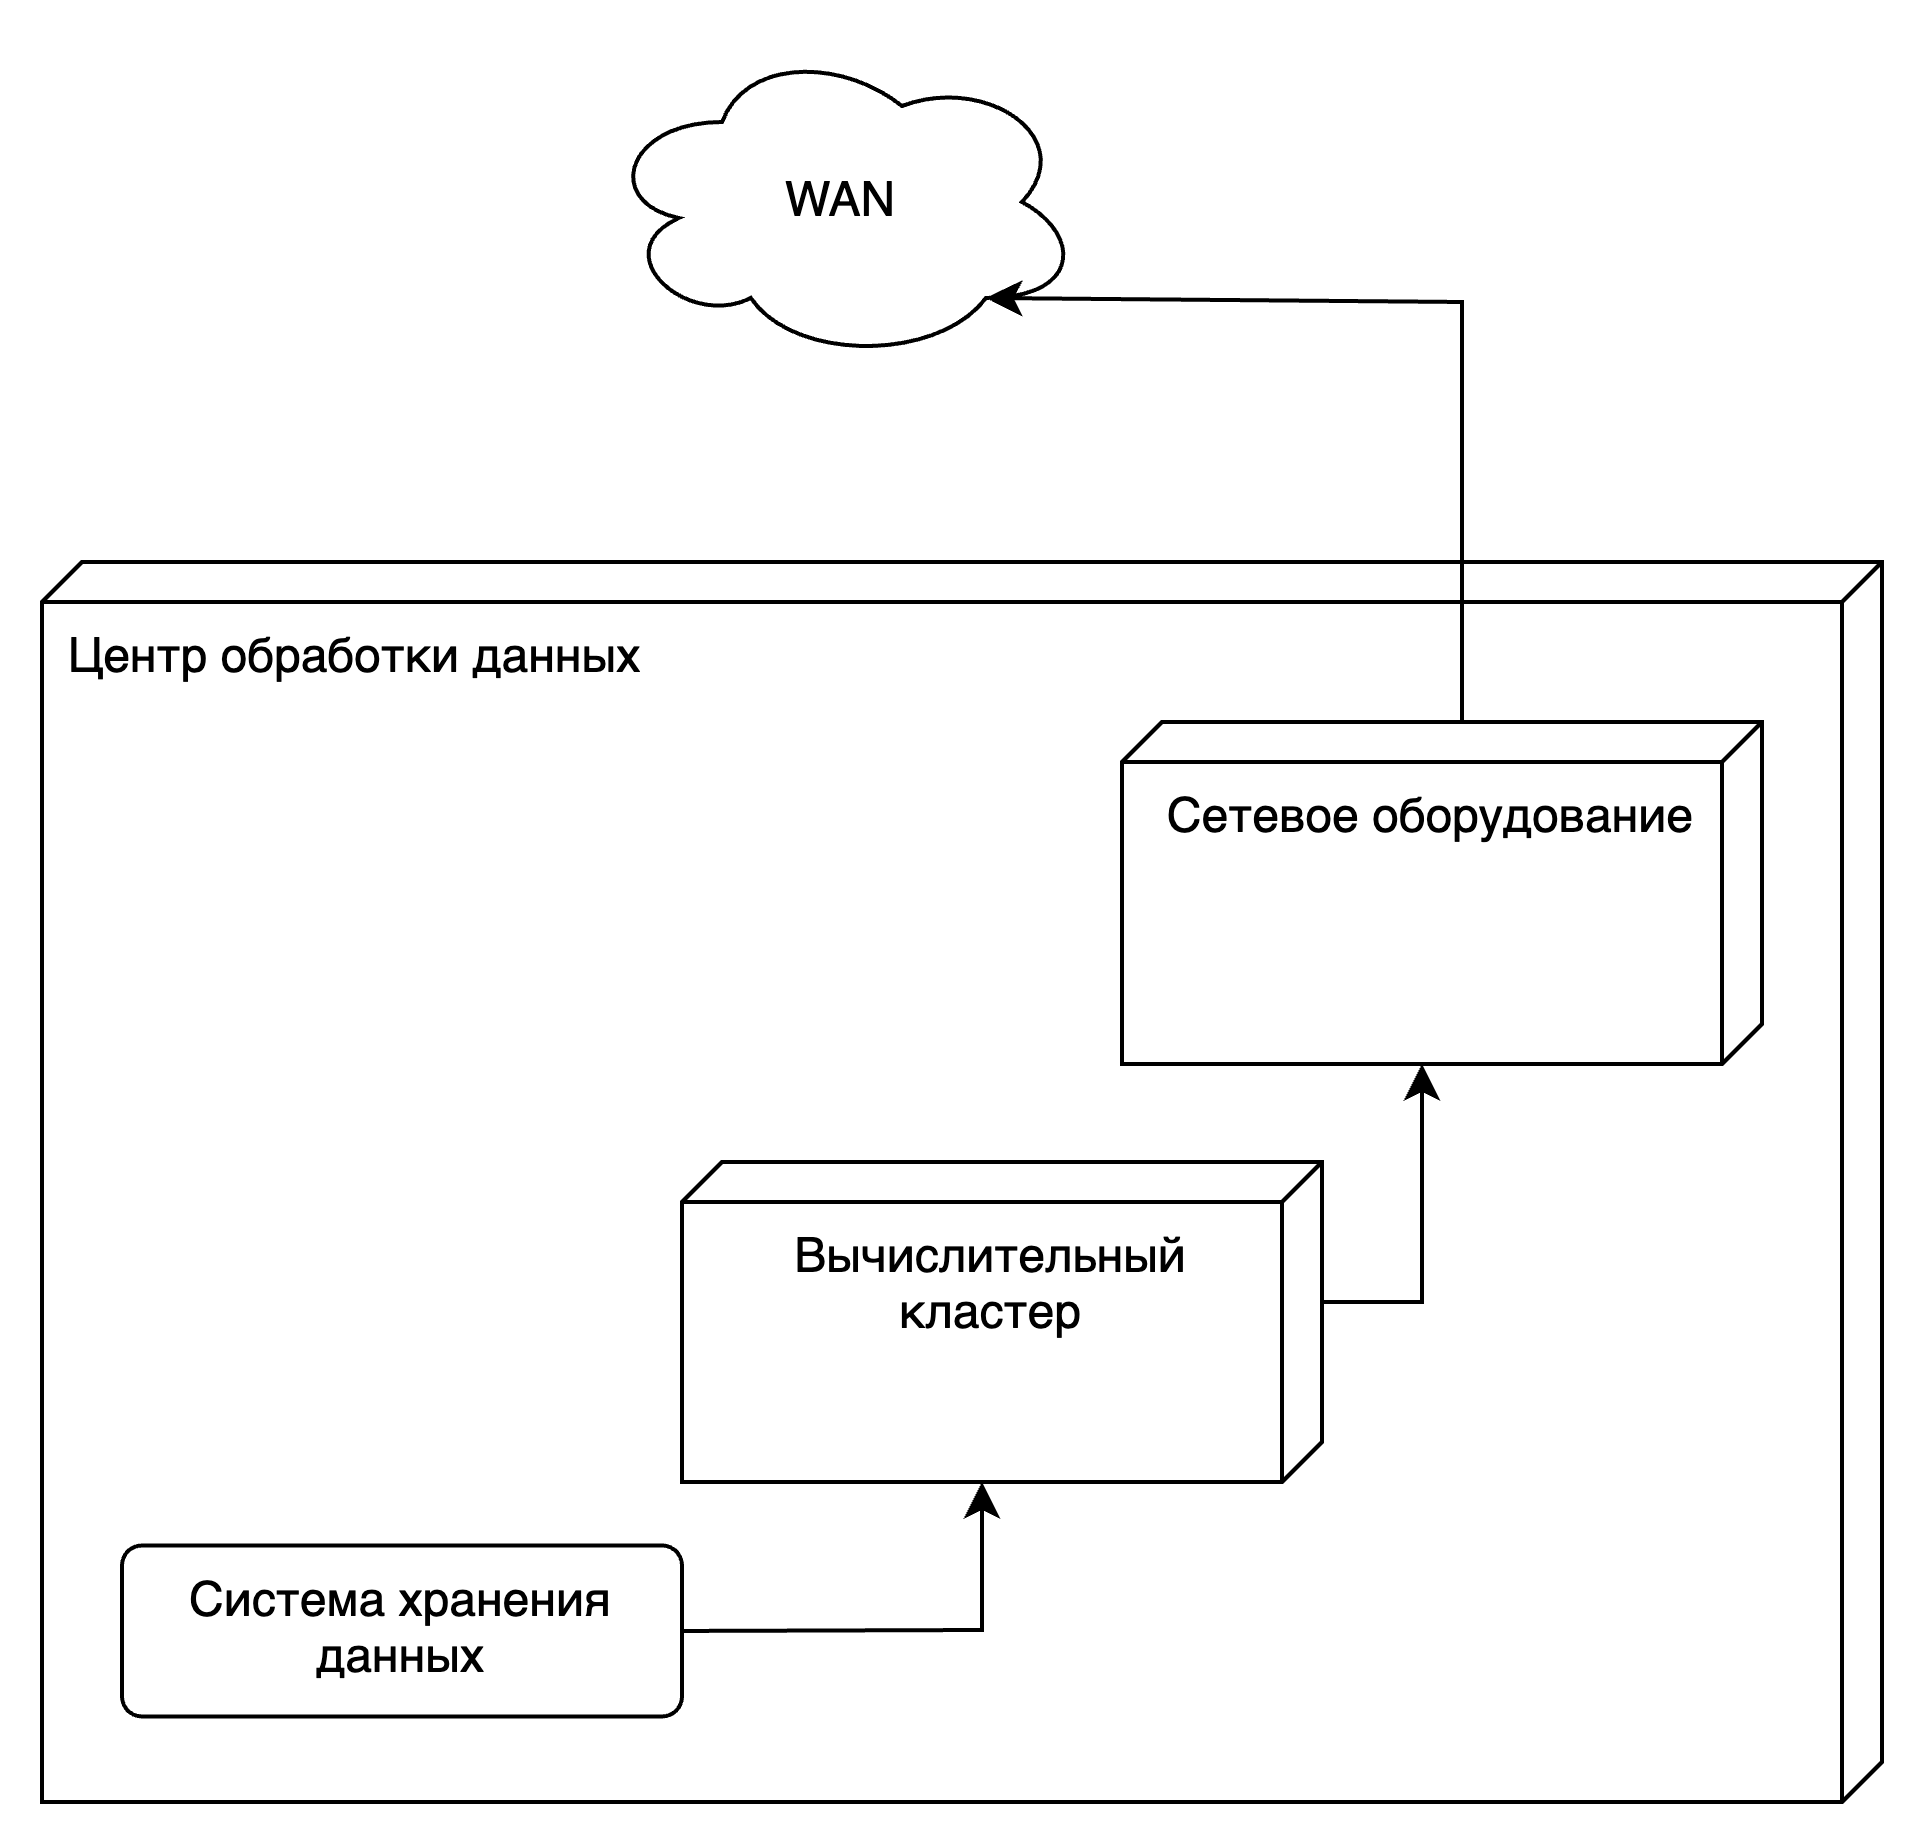
\includegraphics[width=0.7\textwidth]{infra1.png}
  \caption{UML Диаграмма развертывания ИТ-инфраструктуры}
  \label{fig:infra1}
\end{figure}

\subsection{Анализ вариантов компонентов ИТ-инфраструктуры}

В данном разделе произведен анализ возможных компонентов ИТ-инфраструктуры,
которые могут быть использованы в проектируемой инфраструктуре. Основными
компонентами являются серверы, системы хранения данных, сетевое оборудование,
системы резервного копирования и восстановления и системы виртуализации.

Основным критерием для инфраструктуры модуля потребительского кредитования
является отказаустойчивость, безопасность хранения данных и возможность
масштабирования. В связи с этим основные модули инфрастуктури имеют дубликаты
физических компонентов.

Анализ серверов показывает, что для проектируемой инфраструктуры хорошим решением
является использование сервера средней мощности производителя пристутвивующего
в реестре минцифры РФ, что упрощает поиск и содержвание персонала для
обслуживания. Под указанные критерии подходит производитель оборудования <<Гравитон>> \cite{graviton-site}.
У произаводителя имеется широкий выбор серверов, которые поддерживают
разные конфигурации, наиболее подходящим является Сервер «Гравитон» С2122ИУ \cite{graiton-server-s2122iu}.
Данный эземпляр имеет большой потенциал для увеличения объема оперативной памяти,
в отличие от других серверов данной категории, поддерживает до двух процессоров Intel
Xeon. Поддерживает горячую замену блоков питания и вентиляторов, имеет встроенный
модуль управления BMC и полностью соответствует требованиям регуляторов.
Технические характеристики сервера приведены в Таблице\;\ref{tab:graviton_s2122iu}.

\begin{tabularx}{\textwidth}{|l|X|}
  \caption{Технические характеристики сервера Гравитон С2122ИУ\label{tab:graviton_s2122iu}}                                                                                                                \\
  \hline
  Параметр                             & Значение                                                                                                                                                          \\\hline
  \endfirsthead
  \caption*{Продолжение таблицы~\ref{tab:graviton_s2122iu}}                                                                                                                                                \\
  \hline
  Параметр                             & Значение                                                                                                                                                          \\\hline
  \endhead
  \endfoot
  \endlastfoot

  Процессор                            & До 2× Intel Xeon Gold 4-го или 5-го поколения (TDP до 150 Вт)                                                                                                     \\\hline
  Сокет                                & 2× LGA 4677                                                                                                                                                       \\\hline
  Чипсет                               & Intel C741                                                                                                                                                        \\\hline
  Оперативная память                   & До 8 ТБ DDR5; 32 слота DIMM                                                                                                                                       \\\hline
  Поддерживаемые модули памяти         & RDIMM: 8/16/32/64 ГБ; LRDIMM: 64/128/256 ГБ                                                                                                                       \\\hline
  Форм-фактор                          & 2U, стойка 19"                                                                                                                                                    \\\hline
  Дисковая подсистема                  & Передняя панель: 8× 3.5" SAS/SATA/NVMe U.2 + 4× 3.5" SAS/SATA; Задняя панель (опционально): до 4× 2.5" SATA/SAS; 2× M.2 (2280/22110 PCIe 4.0 x4); microSD для BMC \\\hline
  Слоты расширения                     & 2× PCIe 4.0 x8 (низкопрофильные, опционально); 2× PCIe 5.0 x16 (полнопрофильные); 4× PCIe 5.0 x8 (полнопрофильные); OCP NIC                                       \\\hline
  Сетевые интерфейсы                   & Выделенный порт управления (1 Гбит/с RJ-45); 1× OCP 3.0                                                                                                           \\\hline
  Порты ввода-вывода (передняя панель) & Кнопка включения питания; UID-кнопка; 2× USB 3.0; Индикаторы: питания, сетевой активности, UID, состояния системы                                                 \\\hline
  Порты ввода-вывода (задняя панель)   & 1× COM4; 1× RJ-45; 1× VGA; 2× USB 3.0; UID-кнопка; Кнопка сброса                                                                                                  \\\hline
  Модуль управления                    & BMC Aspeed AST2600; Поддержка IPMI 2.0 + iKVM; Выделенный порт IPMI (RJ-45)                                                                                       \\\hline
  Операционные системы                 & Astra Linux, BaseALT, ROSA, RedOS                                                                                                                                 \\\hline
  Система охлаждения                   & 4× 80 мм вентиляторов с горячей заменой                                                                                                                           \\
  Блоки питания                        & 2× 800–2000 Вт, 80+ Platinum, с поддержкой горячей замены                                                                                                         \\\hline
  Безопасность                         & Intrusion Switch                                                                                                                                                  \\\hline
  Габариты (Д×Ш×В)                     & 763 × 447 × 87 мм                                                                                                                                                 \\\hline
\end{tabularx}

Количество физических серверов в проектируемой инфраструктуре составляет три, это позволит
наиболее корректно сформировать отказаустойчивый и высокодоступный кластер в паре с
системой витруализации zVirt.

Система хранения данных (СХД) является наиболее важным звеном в инфраструктуре внутри ЦОД
и отвечает за хранение персональных данных клиентов, их кредитной истории и данных сервисов.

Посколько общеприянтой хорошей практикой является использование одного вендора для всех
компонентов инфраструктуры, так как это позволяет избежать проблем с совместимостью и
обеспечить более простое администрирование. Исходя из этого, в качестве системы хранения
данных выбрана СХД «Гравитон» СХ424И24БМ-РЭ. К конкурентным преимуществам данной модели
можно отнести гибкую мультипротокольную архитектуру, возможноть реализации сложных
уровней RAID и поддержка WORK (write once, read many), что подходит для хранения
персональных данных клиентов, программное обеспечение RAIDIX, которая является
Россйской разработкой и имеет все необходимые сертификаты. Так же не менее важной
особенностью является поддержка горячей замены дисков, блоков питания и вентиляторов.
Выбранный СХД поддерживает до 24 дисков формата 2.5"/3.5", чего достаточно для организации
отказаустойчивого RAID и учета роста объема данных, это определяет целесообразность
использования одного экземпляра.

\begin{tabularx}{\textwidth}{|l|X|}
  \caption{Технические характеристики СХД Гравитон СХ424И24БМ-РЭ\label{tab:graviton_skh424i24bm}}                                                                                                             \\
  \hline
  Параметр                                        & Значение                                                                                                                                                  \\\hline
  \endfirsthead
  \caption*{Продолжение таблицы~\ref{tab:graviton_skh424i24bm}}                                                                                                                                               \\
  \hline
  Параметр                                        & Значение                                                                                                                                                  \\\hline
  \endhead
  \endfoot
  \endlastfoot

  Форм-фактор                                     & 4U, установка в 19" стойку                                                                                                                                \\\hline
  Процессоры                                      & 4× Intel Xeon Gold Gen2                                                                                                                                   \\\hline
  Оперативная память                              & До 4 ТБ                                                                                                                                                   \\\hline
  Контроллеры                                     & Двухконтроллерная конфигурация (Active-Active)                                                                                                            \\\hline
  Дисковая подсистема                             & 24× 2.5"/3.5" SSD/HDD с поддержкой горячей замены                                                                                                         \\\hline
  Максимальная емкость хранения                   & До 2 ПБ                                                                                                                                                   \\\hline
  Поддерживаемые интерфейсы дисков                & SAS, NL-SAS, SATA                                                                                                                                         \\\hline
  Поддерживаемые уровни RAID                      & 0, 1, 5, 6, 7.3, 10, 50, 60, 70, N+M                                                                                                                      \\\hline
  Максимальное количество дисков в RAID           & 64                                                                                                                                                        \\\hline
  Максимальное количество LUN                     & 447                                                                                                                                                       \\\hline
  Поддерживаемые файловые протоколы               & SMB v2/v3, NFS v3/v4, AFP, FTP                                                                                                                            \\\hline
  Поддерживаемые блочные протоколы                & FC 8/16/32 Гбит/с, iSCSI/iSER 10/25/40/100 Гбит/с, InfiniBand SRP 20/40/56/100 Гбит/с, SAS 12 Гбит/с                                                      \\\hline
  Поддерживаемые платформы виртуализации          & VMware ESXi, Microsoft Hyper-V, KVM, XenServer, Proxmox VE, RHEV                                                                                          \\\hline
  Поддерживаемые операционные системы инициаторов & Windows Server 2016/2019/2022, Ubuntu 18.04/20.04/22.04, RHEL 7.x/8.x, Astra Linux 1.7, Альт Сервер 10, РЕД ОС 7.3, macOS                                 \\\hline
  Программное обеспечение СХД                     & RAIDIX 5.X                                                                                                                                                \\\hline
  Дополнительные функции                          & WORM, упреждающая и частичная реконструкция, защита от скрытого повреждения данных, SSD-кэш, QoSmic, SAN Optimizer                                        \\\hline
  Сетевые интерфейсы                              & до 32× 10 Гбит/с Ethernet, до 16× 32 Гбит/с Fibre Channel, до 32× 8/16 Гбит/с Fibre Channel, 4× 1 Гбит/с RJ-45, выделенный порт управления 1 Гбит/с RJ-45 \\\hline
  Блоки питания                                   & 2× 1300 Вт, 80+ Platinum, с поддержкой горячей замены                                                                                                     \\\hline
  Температурный диапазон                          & Эксплуатация: 10°C ~ 35°C, хранение: -20°C ~ 45°C                                                                                                         \\\hline
\end{tabularx}

Операционная система RAIDX \cite{raidix-web} используемая в СХД позволяет реализовать
автоматический перенос на разные кровни хранения. Все уровни хранения используемые в
инфраструктуре представлены в Таблице\;\ref{tab:DSS_storage_levels}.

\begin{tabularx}{\textwidth}{|l|X|X|X|X|}
  \caption{Уровни хранения данных СХД\label{tab:DSS_storage_levels}}                                                                                                                     \\
  \hline
  Уровень хранения данных & Тип Дисков           & Назначение                           & Модель             & Описание модели                                                           \\\hline
  \endfirsthead
  \caption*{Продолжение таблицы~\ref{tab:DSS_storage_levels}}                                                                                                                            \\
  \hline
  Уровень хранения данных & Тип Дисков           & Назначение                           & Модель             & Описание модели                                                           \\\hline
  \endhead
  \endfoot
  \endlastfoot

  Горячие данные          & 4–6 × SSD SAS / NVMe & Базы данных, кэш, логи               & Intel D3-S4610     & Стабилен в работу, имеет большой ресурс DWPD и сертиф ицирован под RAIDIX \\\hline
  Операционные данные     & 8–12 × HDD 10K SAS   & Справочники, актуальные документы    & Seagate Exos 10K.2 & Лучшие по цене и надежности, широко поддер живаются                       \\\hline
  Архив/бэкап             & 8–12 × NL-SAS 7.2K   & Архивы, резервы, исторические данные & Seagate Exos X16   & Очень популярные, высокая плотность, поддержка PowerChoice                \\\hline
\end{tabularx}

\subsection{Системное программное обеспечение}

% На серверы в ЦОД установалена система виртуализации <<ProxMox>> \cite{prox-mox}, которая позволяет
% объеденить все серверы в кластер, этим обеспечивает отказаустойчивость, высокую
% доступность и возможность управления всеми ресурсами централизованно из единой
% консоли. Внутри кластера настроена распределенная система хранения данных <<Ceph>> \cite{ceph},
% которая позволяет использовать все SAS и NVME диски в кластере как единое
% хранилище данных, что позволяет обеспечить высокую скорость доступа к данным
% и отказаустойчивость. <<Ceph>> хорошо интегрируется с <<Proxmox>> и поддерживает
% отказоустойчивость и балансировку нагрузки.

% Так как ЦОД предназнчен не только для хранения, но и для обработки данных критически
% важных сервисов, то на внутри кластера созданы виртуальные машины с операционной
% системой <<ALT Linux>> с использованием части которых сформирован <<Kubernetes>>
% кластер состоящий их нескольких узлов. <<Kubernetes>> позволяет управлять критически
% важными сервисами и приложениями, которые обеспечивают работу модуля потребительского
% кредитования.

% Внутри кластера <<ProxMox>> настрен СУБД <<PostgreSQL>> с политикой репликации
% мастер-слейв, что уменьшает нагрузку на узел и повышает отказаустойчивость и доступность
% данных, так как позволяет читать данные для аналитики с реплики. Как нереляционная база
% данных используется <<MongoDB>>, которая так же настроена внутри отдельной виртуальной
% машины кластера <<ProxMox>>.


% В облаке <<Yandex Cloud>> так же используется <<Kubernetes>> для управления
% всеми сервисами и приложениями, которые обеспечивают работу модуля потребительского.
% Для CRM в используется отедльная виртуальная машина с предустановленной <<1C-Битрикс>>.


\section{Заключение}


% used resources list
\begingroup
\let\itshape\upshape
\sloppy
\raggedright
\printbibliography[title=СПИСОК ИСПОЛЬЗУЕМЫХ ИСТОЧНИКОВ]
\phantomsection
\addcontentsline{toc}{section}{СПИСОК ИСПОЛЬЗУЕМЫХ ИСТОЧНИКОВ}
\endgroup
% used resources list

\end{document}